\chapter{Design}
\label{chap:design}

\section{Architettura}
\label{sec:design-architettura}

Il sistema è strutturato secondo un'architettura client-server a tre livelli, in cui ogni livello è realizzato come modulo indipendente all'interno di un unico progetto multi-modulo. I quattro moduli che compongono il progetto sono \texttt{fmilib}, \texttt{fmu-kt}, \texttt{backend} e \texttt{frontend}, ciascuno con responsabilità ben delimitate e dipendenze unidirezionali.

Il modulo \texttt{fmilib} costituisce la base della catena di dipendenze: si occupa della compilazione della libreria nativa \emph{FMILib} e ne espone gli artefatti (header C e librerie condivise) agli strati superiori. Questa scelta isola completamente la toolchain di compilazione dal resto del progetto Kotlin, rendendo il confine tra codice nativo e codice multipiattaforma esplicito e controllato.

Il modulo \texttt{fmu-kt} costituisce il cuore della logica di dominio. Dipende da \texttt{fmilib} e si occupa di tutto ciò che riguarda il ciclo di vita degli FMU: caricamento del file, parsing dell'XML descrittivo, invocazione della libreria nativa per l'esecuzione della simulazione, e restituzione dei risultati. Il modulo è compilato come libreria Kotlin Multiplatform per le piattaforme native (Linux x64, macOS ARM64 e Windows x64), consentendo di riutilizzare la logica comune tra le piattaforme e di isolare, nei codici sorgente specifici, le parti che richiedono comportamenti differenziati — in particolare la fase di preelaborazione degli FMU su macOS ARM, che richiede la ricompilazione del modello.

Il modulo \texttt{backend} implementa un server HTTP REST che espone le funzionalità di \texttt{fmu-kt} come API consumabile dal frontend, è anch'esso un modulo Kotlin Multiplatform con target nativi. Il server espone endpoint per il caricamento del file FMU, l'inizializzazione, la lettura dei metadati e l'esecuzione della simulazione.

Il modulo \texttt{frontend} realizza l'interfaccia utente web. Il frontend comunica con il backend, permettendo così all'utente di interagire con gli endpoint esposti e di avere una visualizzazione grafica delle informazioni e dei risultati della simulazione.

% TODO: inserire diagramma architettura
\begin{figure}[h]
  \centering
  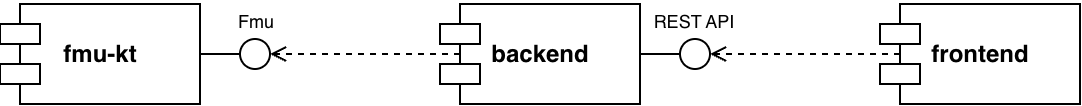
\includegraphics[width=0.85\textwidth]{figures/diagramma-tirocinio.png}
  \caption{Diagramma rappresentante relazione tra i moduli dell'applicativo.}
  \label{fig:architettura}
\end{figure}

Questa scelta disaccoppia completamente i tre processi: il backend può essere avviato indipendentemente, testato in isolamento tramite client HTTP standard, e in futuro potrebbe essere esposto su rete senza modifiche architetturali. Il frontend non conosce nulla della logica FMU; conosce solo i contratti delle API REST. Mentre il modulo \texttt{fmu-kt} funge da libreria indipendente, dunque può essere esportata per essere usata in altri progetti.

Una conseguenza rilevante di questa architettura è la separazione netta tra la parte del sistema che richiede accesso nativo — \texttt{fmu-kt} e \texttt{backend}, che devono interagire con la libreria C e con il filesystem — e la parte puramente applicativa del frontend, che rimane nel dominio Kotlin puro. Questo ha guidato la decisione di non integrare \texttt{fmu-kt} direttamente nel frontend, evitando di contaminare il modulo UI con dipendenze native.

\section{Design di dettaglio}
\label{sec:design-dettaglio}

Le sezioni seguenti approfondiscono le scelte di design dei tre componenti principali del sistema, seguendo lo stesso ordine delle dipendenze architetturali descritte in precedenza: si parte dall'interfacciamento con le librerie native, che costituisce il fondamento su cui si appoggiano gli strati superiori, per risalire al backend — che orchestra la logica di dominio ed espone i servizi verso l'esterno — fino al frontend, responsabile della presentazione e dell'interazione con l'utente.

Per ciascun componente vengono discusse le scelte progettuali significative, con particolare attenzione ai confini tra codice condiviso e codice specifico per piattaforma, e alle motivazioni che hanno guidato la separazione delle responsabilità.

\subsection{Interfacciamento con librerie native}
\label{subsec:design-native}

Il modulo \texttt{fmu-kt} è il componente del sistema responsabile di tutta l'interazione con la libreria nativa FMILib. Il suo design è orientato ad astrarre la complessità di basso livello esposta dalla libreria C, presentando agli strati superiori un'interfaccia di alto livello che non richiede alcuna conoscenza dei dettagli nativi.

Il punto di accesso esterno al modulo è \texttt{FmuService}, un'interfaccia che espone le operazioni disponibili sugli FMU: caricamento, lettura dei metadati e avvio della simulazione. Questa scelta consente al backend di dipendere esclusivamente dal contratto dell'interfaccia, rendendo il modulo sostituibile e facilmente testabile tramite implementazioni fittizie.
Ulteriori funzionalità potranno essere introdotte in futuro aggiungendo nuovi
metodi all'interfaccia e le relative implementazioni, senza alterare la
struttura generale del modulo.

L'implementazione concreta del servizio delega la gestione del modello a\\\texttt{FmuManager}, un componente che orchestra l'intero ciclo di vita di un FMU attraverso tre manager specializzati, ciascuno con una responsabilità ben delimitata:

\begin{itemize}
  \item \textbf{FmuLifecycleManager}: si occupa dell'apertura e della chiusura dell'FMU, gestendo l'allocazione e il rilascio delle risorse associate.
  \item \textbf{InfoManagerFmu}: estrae i metadati del modello — nome, autore, versione, variabili disponibili e parametri dell'esperimento predefinito — interrogando direttamente le strutture dati native.
  \item \textbf{SimulationManager}: gestisce la configurazione e l'esecuzione della simulazione raccogliendo i risultati e restituendoli in un formato indipendente dalla libreria nativa.
\end{itemize}

Questi tre manager sono gli unici componenti del sistema che interagiscono direttamente con FMILib. Concentrare questo confine in un insieme ristretto e ben identificato di classi rende il sistema più manutenibile: eventuali cambiamenti nell'API nativa o l'adozione di una libreria FMI alternativa richiederebbero modifiche localizzate nei manager, senza propagarsi al resto dell'architettura.

Prima che un FMU possa essere caricato, è necessaria una fase di preparazione del file che ne garantisce la compatibilità con la piattaforma corrente. Questa responsabilità è affidata al \texttt{FmuPreprocessor}, un componente separato la cui implementazione varia a seconda della piattaforma target. La sua interfaccia è definita nel source set comune, mentre le implementazioni specifiche risiedono nei source set di piattaforma, seguendo il meccanismo \texttt{expect}/\texttt{actual} di Kotlin Multiplatform. In questo modo la logica di preparazione dell'FMU rimane completamente trasparente agli strati superiori.

\subsection{Backend multipiattaforma}
\label{subsec:design-backend}

\subsection{Frontend multipiattaforma}
\label{subsec:design-frontend}